% Polycopie pour les etudiants

\documentclass[handout]{beamer}[10pt, usepdftitle=false]
%%\usepackage[printwatermark]{xwatermark}
\usepackage{pgfpages}
\pgfpagesuselayout{6 on 1}[a4paper,border shrink=5mm] % 4 par 4

% NE PAS OUBLIER DE BAISSER A QUALITE DU POLYCOPIE!: gs -sDEVICE=pdfwrite -dCompatibilityLevel=1.4 -dPDFSETTINGS=/ebook -dNOPAUSE -dQUIET -dBATCH -sOutputFile=small.pdf big.pdf

% Mes slides pour le cours
%\documentclass{beamer}[10pt, usepdftitle=false handout]


\beamertemplatenavigationsymbolsempty

\usepackage[T1]{fontenc}
\usepackage[]{algorithm2e}
\usepackage{multimedia}
\usepackage{gensymb}
\usepackage{textcomp}
%\usepackage{tikz}

\usepackage{listings}

%\usepackage{background}
%\backgroundsetup{
%    placement=center,
%    scale=5,
%    color=lightgray,
%    contents={PAUL BLONDEL},
%    opacity=0.2
%}
%\setbeamertemplate{background}{\BgMaterial}


%\usepackage[font=small,labelfont=bf]{caption} 

\usetheme{Boadilla}

\title{Introducton to Data Engineering 1}
\author[]{Paul Blondel}
\institute[]{UTSEUS, Shanghai}
\date[]{March 30st, 2021}

\usepackage[style=british]{csquotes}


\def\signed #1{{\leavevmode\unskip\nobreak\hfil\penalty50\hskip1em
  \hbox{}\nobreak\hfill #1%
  \parfillskip=0pt \finalhyphendemerits=0 \endgraf}}

\newsavebox\mybox
\newenvironment{aquote}[1]
  {\savebox\mybox{#1}\begin{quote}\openautoquote\hspace*{-.7ex}}
  {\unskip\closeautoquote\vspace*{1mm}\signed{\usebox\mybox}\end{quote}}


\setbeamertemplate{headline}
{
  \leavevmode%
  \hbox{%
  \begin{beamercolorbox}[wd=1.0\paperwidth,ht=2.25ex,dp=1ex,center]{author in head/foot}%
    \usebeamerfont{author in head/foot}\insertsubsection
  \end{beamercolorbox}}%
  \vskip0pt%
}


\setbeamertemplate{footline}
{
  \leavevmode%
  \hbox{%
  \begin{beamercolorbox}[wd=.5\paperwidth,ht=2.25ex,dp=1ex,center]{author in head/foot}%
    \usebeamerfont{author in head/foot}\insertsection
  \end{beamercolorbox}%
  \begin{beamercolorbox}[wd=.5\paperwidth,ht=2.25ex,dp=1ex,center]{title in head/foot}%
    \usebeamerfont{title in head/foot} \inserttitle \hspace*{2em}  \insertframenumber{} / \inserttotalframenumber\hspace*{2ex} 
  \end{beamercolorbox}}%
  \vskip0pt%
}

\AtBeginSection[]
{
   \begin{frame}
    \tableofcontents[ 
    currentsection] 
   \end{frame}
}

\begin{document}
	{
	\setbeamertemplate{footline}{
  	\leavevmode%
  	\hbox{%
  	\begin{beamercolorbox}[wd=.5\paperwidth,ht=2.25ex,dp=1ex,center]{author in head/foot}%
  	\end{beamercolorbox}%
  	\begin{beamercolorbox}[wd=.5\paperwidth,ht=2.25ex,dp=1ex,center]{title in head/foot}%
  	\end{beamercolorbox}}%
  	\vskip0pt%	
	} 
	\begin{frame}
	\titlepage
	\end{frame}

	\begin{frame}
	
	\begin{aquote}{Daniel Keys Moran}
You can have data without information, but you cannot have information without data.
	\end{aquote}	
	\end{frame}

	\begin{frame}
		\tableofcontents
	\end{frame}
	}

	\addtocounter{framenumber}{-3}

	\section{Introduction}	

    \begin{frame}[label=(first)]
	Since the beginning of computers, data is a key component:
	\begin{itemize}
	\item{Operating systems are stored as data in the hard-drive and loaded in the main memory}
	\item{Computer users' data are stored on hard-drive, optical discs, etc}
	\end{itemize}	
	\vspace*{0.6em}	
	
	Because, with computers, data can not only be read but also easily written and erased, one can...
	\begin{itemize}
	\item{...install/uninstall a software}
	\item{...update the OS}
	\item{...write a word document}
	\item{...have a custom system and a personal experience}
	\end{itemize} 
	\vspace*{0.6em} 	
	
	\begin{block}{The software era}
	Compared to an old-school calculator: the flexibility to access and edit the data made a great difference and opened the era of software creation.
	\end{block}	
	\end{frame}
	
	\begin{frame}	
	
	However nowadays, data is more than just your operating system, all your software and some word documents...
	\vspace*{1.0em}	
	
	There have been a series of recent discoveries and breakthroughs making possible the \textbf{extraction, the storage, the pre-processing and the processing, the analysis and the building of statistical and Machine Learning models on bigger and bigger amounts of data}. 
	\vspace*{0.6em}
	
	
	\begin{block}{The era of data}
	Brand new applications are nowadays unlocked thanks to that: making the engineering of data a top priority in most companies worldwide.
	\end{block}
	

	\begin{alertblock}{First thing first!}
	Before manipulating petabytes of data, let's understand how to change information into data, and first, how to store data into... the memory!
	\end{alertblock}			
			
    \end{frame}


\section{Memory}
	\subsection{Different memories for different usages}
	
	\begin{frame}

	Different types of memory:
	\begin{itemize}
	\item {CPU registers
		\begin{itemize}
			\item{Stores data directly used by the CPU (instructions, memory addresses, program counter, accumulator, etc.)}
		\end{itemize}			
	}
	\item {Cache Memory
		\begin{itemize}
			\item{Temporary stores copies of the data from frequently used and/or nearby main memory locations}
		\end{itemize}			
	}
	\item {Main Memory (Random-access memory or RAM)
		\begin{itemize}
			\item {Stores running softwares and opened documents}	
		\end{itemize}			
	}
	\item {Mass Storage Memory 
		\begin{itemize}
			\item {Stores installed softwares and all documents}
			\item {Two main technologies on the market: 
				\begin{itemize}
					\item {Hard-disk drive (HDD) (invented in 1954)}
					\item {Solid-state drive (SSD) (invented in 1978)}
				\end{itemize}
			}
		\end{itemize}			
	}
	\item {Optical discs}
	\item {GPU memory units}	
	\end{itemize}
	
	\end{frame}


\subsection{How it works?}

	\begin{frame}
	
	\begin{itemize}
		\item {CPU Registers 
			\begin{itemize}
				\item{Y1, Y2, PSW, Z: registers used to store operation values, store computed value and remain}
				\item{RI, CO: registers storing instructions}	
				\item{RAD: register storing memory address}
				\item{RDO, general registers: registers storing data}		
			\end{itemize} 
			
	\begin{figure}
		\includegraphics[scale=0.030]{images/cpu.png} 
     	\vspace*{-0.5em}
		\caption{Simple CPU architecture}
	\end{figure}				
	}
	
	\end{itemize}
	
	\end{frame}

	\begin{frame}
	
	\begin{itemize}
		\item {Cache Memory
			\begin{itemize}			
				\item{Located between the Computer Processing Unit (CPU) and the main memory}
				\item{Help reducing the number of accesses to the main memory, reducing the overall memory access time
					\begin{itemize}
						\item{By temporary storing copies of the data from frequently used and/or nearby main memory locations}		
					\end{itemize}									
				}
			\end{itemize} 
			
		\begin{figure}
			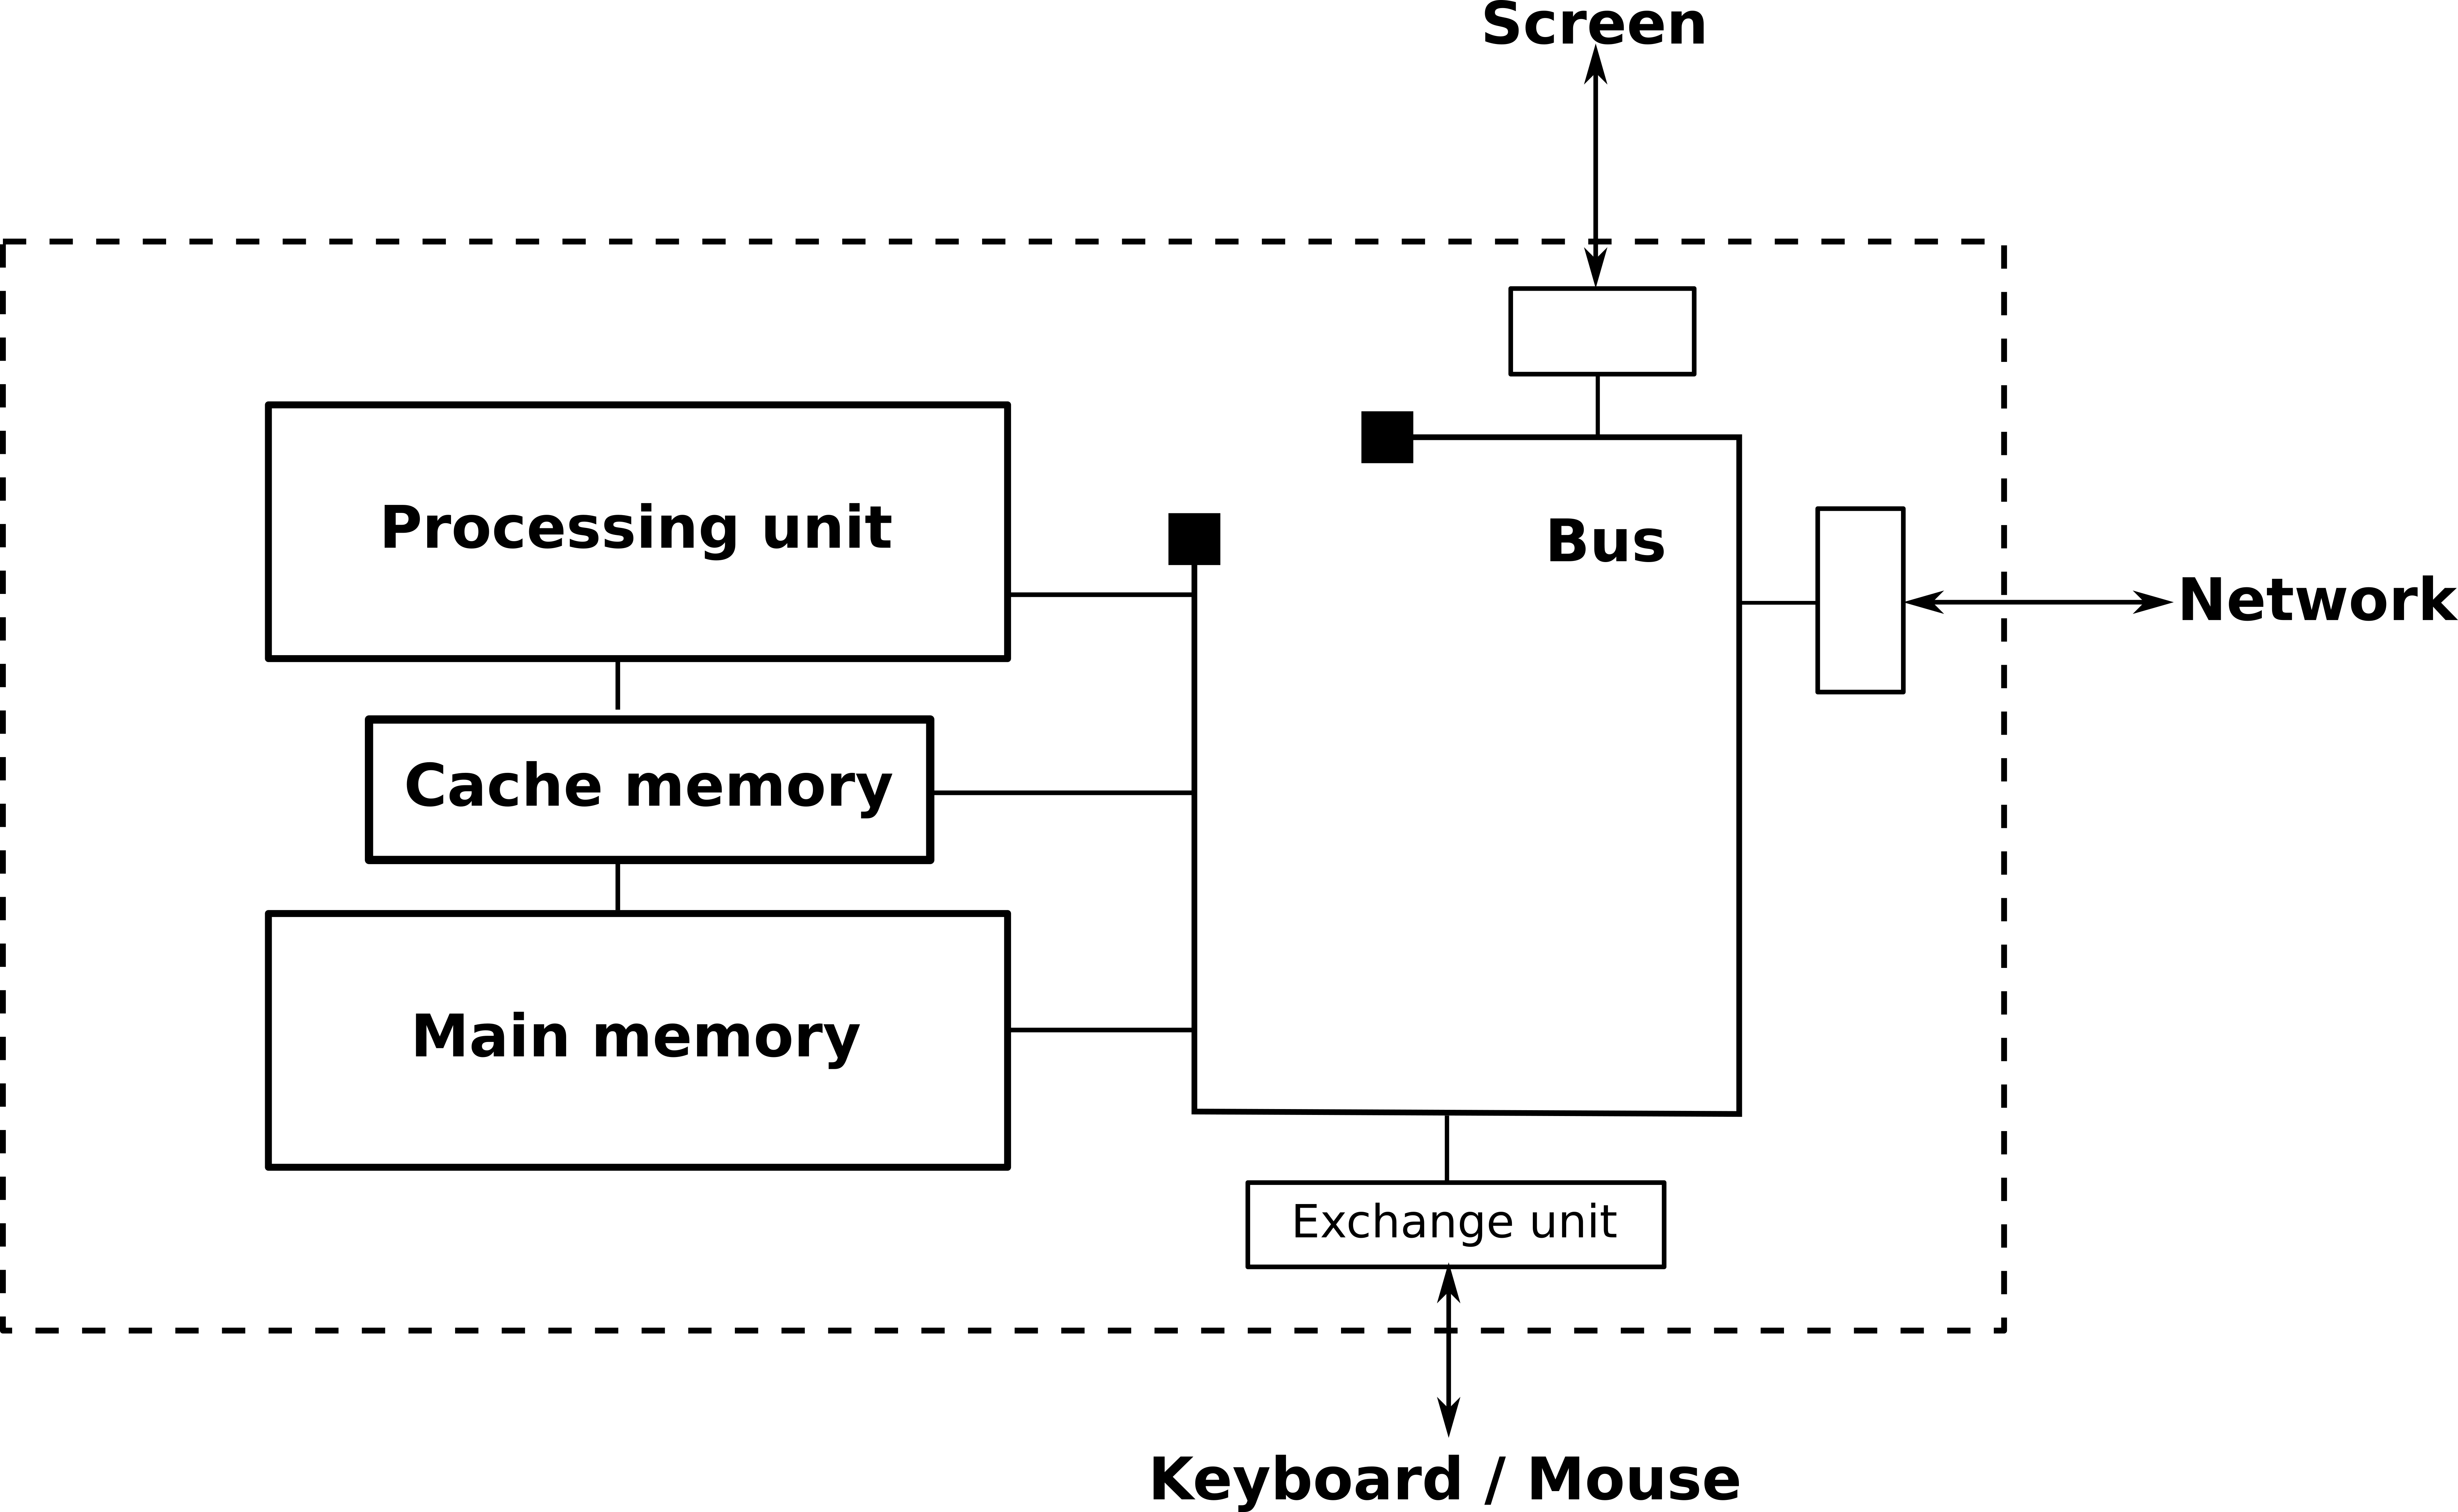
\includegraphics[scale=0.06]{images/von_neumann.png} 
     		\vspace*{-0.5em}
			\caption{Von Neumann computer architecture}
		\end{figure}		
		}
	
	\end{itemize}
	
	\end{frame}

	\begin{frame}    
    
   	\begin{itemize}
   	
	\item {RAM (Main Memory)
		\begin{itemize}
			\item {All the data is stored in an array of storage cells}
			\item {1 bit = 1 storage cell (DRAM: bit stored in a capacitor)}
			\item {Volatile memory: need electric power for storage}
		\end{itemize}
		\begin{figure}[t]
		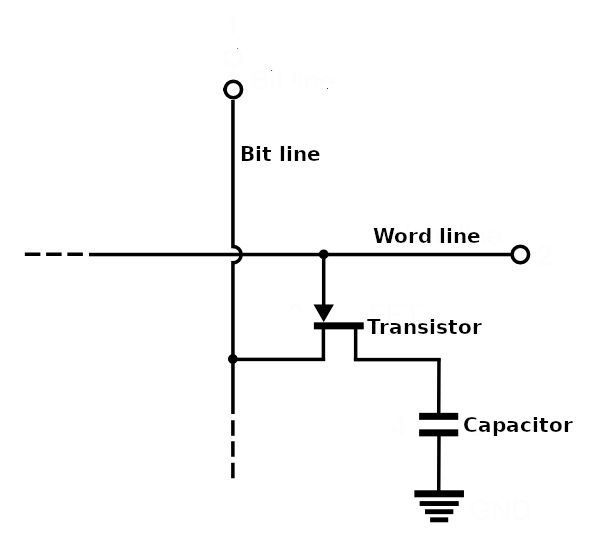
\includegraphics[scale=0.5]{images/ddr_cell.png}
		\vspace*{-0.9em}
		\caption{DRAM memory cell}
		\centering
		\end{figure}
		}
	\item {HDD (Mass Storage Memory)
		\begin{itemize}
			\item {All the data is stored in disks of ferromagnetic material}
			\item {1 bit = direction of magnetic field lines}			
		\end{itemize}			
				
		\begin{figure}
		\begin{tabular}{cc}
		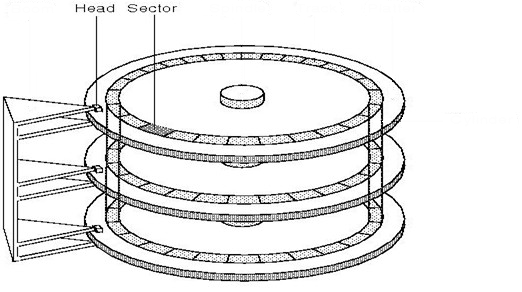
\includegraphics[scale=0.9]{images/hdd_disks.png} &	
		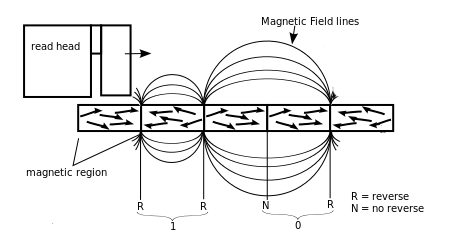
\includegraphics[scale=0.9]{images/hdd_magnetic.png} \\
		\end{tabular}
		\vspace*{-0.5em}
		\caption{Left: disks of ferromagnetic material right: magnetic field lines}
		\end{figure}		
	}						
	
	\end{itemize}
	
	% the bit of memory is stored in the capacitor, but the capacitor leaks, so it has to be refreshed  each time, that why we call it dynamic 	
	% current in the transistor: the bit line receive the value of the capacitor
	% current in the bit line with 1: we write 1, with 0, we write 0	
	
		   
    \end{frame}
    	
	\begin{frame}
	
	\begin{itemize}
		\item {SSD (Mass Storage Memory)
			\begin{itemize}
				\item{All the data is stored in an array of floating-gate transistors}
				\item{No mechanical moving component = faster}
				\item{Non-volatile memory: electrons trapped in the floating-gate (surrounded by oxide layers)}
						
			
			\end{itemize} 
			
			\begin{figure}
				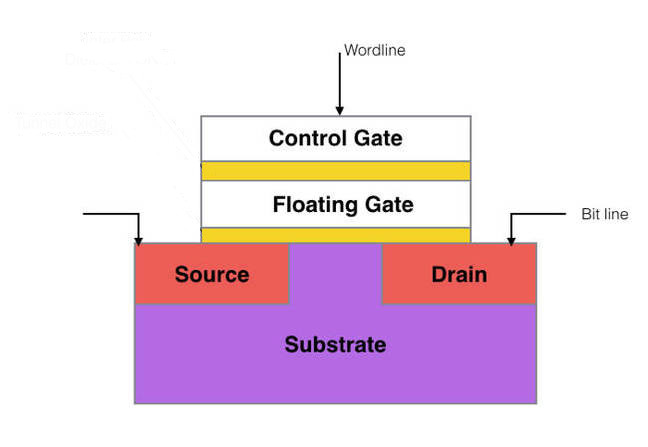
\includegraphics[scale=0.2]{images/floating_gate_flash_cell.jpg} 
     			\vspace*{-0.5em}
				\caption{Floating gate transistor cell}
			\end{figure}			
			
			% The bit is stored in the floating gate, when there is not current in the bit line the bit is tored in the floating gate
			
			}
	
	\end{itemize}
	
	
	\end{frame}  
	
	\begin{frame}
	
	\begin{itemize}
		\item {Optical Discs
			\begin{itemize}
				\item{Mechanical moving component, disc moving and laser head reading}
				\item{Non-volatile memory: bits are "physically" created ("holes" or chemical reactions)}			
			\end{itemize} 
			
		\begin{figure}
			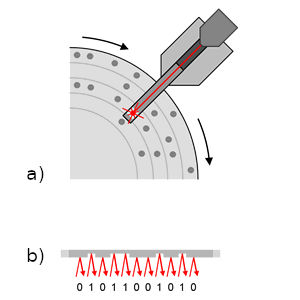
\includegraphics[scale=0.3]{images/optical-disc.png} 
    	 	\vspace*{-0.5em}
			\caption{Reading optical discs}
		\end{figure}			
		
	
		\begin{itemize}
			\item{The laser arm and the disc move alike the HDD mechanism (a)}	
			\item{Bits are represented by pits etched on the disc itself (b)}
		\end{itemize}		
	}
	
	\end{itemize}
	
	\end{frame}	
	
	\begin{frame}
	
	Summary of the main properties of computer memories:
	
	% ajouter CPU registers/Cache Memory/Optical/ etc.
	\begin{center}
	\resizebox{\columnwidth}{!}{
	\begin{tabular}{c | c | c | c | c | c }
		& CPU Registers & Cache & RAM & HDD / SSD & Optical Discs \\ \hline
		Access speed & Ultra fast (1 or few CPU cycles) & Very fast (20000-200000MO/s) & Fast (2000-26600MO/s) & Slow (50-500MO/s) & Very Slow (0.150-3MO/s) \\
		Storage capacity & Ultra low (32/64 bits) & Very low (512KB-8MB) & Low (4-32GB) & High (256GB - 1TB) & Moderate High (700MO-25GB)\\
		Storage property & Volatile & Not Volatile & Volatile &  Not Volatile & Not Volatile  
	\end{tabular}
	}
	\end{center}


	\end{frame}	
	
	\begin{frame}
	
	\begin{figure}
		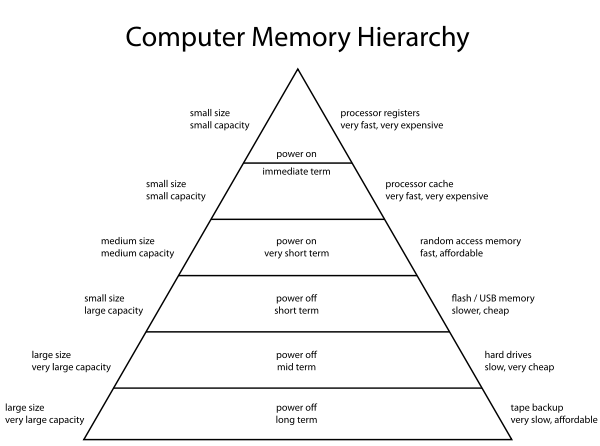
\includegraphics[scale=0.35]{images/memory-hierarchy.png} 
     	\vspace*{-0.5em}
		\caption{The Memory Hierarchy: a trade-off between storage capacity and speed}
	\end{figure}		

	\begin{block}{Notes}
	To optimize the speed of execution: top of the pyramid memories should be use as much as possible! (Require to design your program accordingly).
	\end{block}	
	
	
	\end{frame}	
	
	\begin{frame}
	\begin{columns}[c]
	\column{.5\textwidth}
	GPU memories: a complex assembly:
	\begin{itemize}
		\item{Registers: very fast access, thread, few space}
		\item{Local Memory: slow access, thread, more space}
		\item{Shared Memory: fast access, block, more space}
		\item{Global Memory: slow access, all blocks, more space}
		\item{Constant Memory: fast access, all blocks, more space}
		\item{Texture Memory: fast access, all blocks, read-only}
	\end{itemize} 		
	
	\column{.5\textwidth}	
		\begin{figure}
		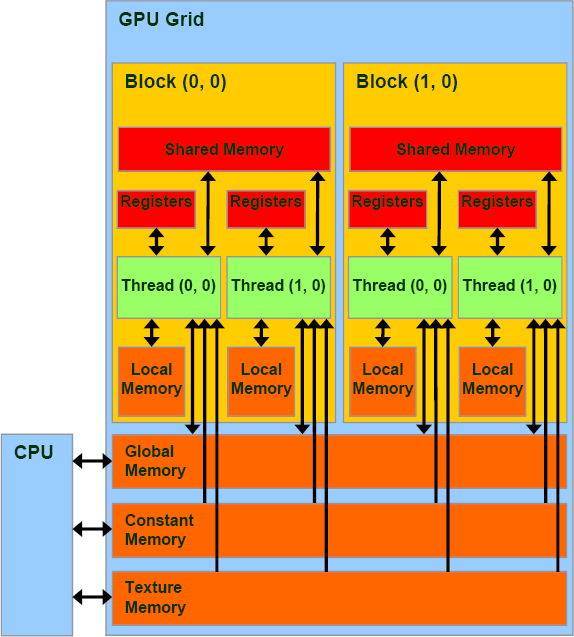
\includegraphics[scale=0.2]{images/cuda-enabled-gpu.png} 
     	\vspace*{-0.5em}
		\caption{Memory units of Nvidia GPUs}
		 \end{figure}
	\end{columns}
	\begin{block}{GPU memories: A more complex trade-off}
	With GPU memory units: a trade-off storage capacity VS access speed VS accessibility. That's why coding optimal code for GPU is hard.	\end{block}
	
	\end{frame}	
	
	\section{Data}	
	
	\subsection{Data, types and properties}	

    \begin{frame}[label=(first)]
	
	\begin{block}{What is data?}
	Data is the result of a measurement
	\end{block}	
			
	Examples: The diameter of the sun is \textbf{1.39 million kilometers}, the temperature of the room is \textbf{30\degree C}, and so on.
	
	\hfill\break
			
	A data ...
			
	\begin{itemize}
	\item {... is \textbf{simple} or \textbf{complex} (composed of simple data)}	
	\item {... has a \textbf{type} (integer, character, and so on)}
	\item {... has a set of authorized \textbf{instructions}}
	\end{itemize}
	
	Examples: 'hello' is a complex data (composed of simple character data), 30\degree C is a simple integer data. 'hello' * 30 is not authorized, but 2 * 30 is.
		 
			
    \end{frame}

	%\section{Data}	
	\subsection{Units}	

    \begin{frame}
    
	The most common units are: 
	\begin{itemize}
		\item{1 bit (0 or 1)}
		\item{1 byte (or octet) = 8 bits}
		\item{1 KB (or KO) = 1000 bytes\footnote{1 KB is sometimes defined as equal to 1024 bytes, but this definition is no longer valid. In 1998, the International Electrotechnical Commission stated that 1 KB = 1000 bytes and that 1024 bytes = 1 KiB (kibibyte).}}
		\item{1 MB (or MO) = $10^6$ bytes = 1000 KB}
		\item{1 GB (or GO) = $10^9$ bytes = $10^6$ KB = 1000 MB}
		\item{1 TB (or TO) = $10^{12}$ bytes}
	\end{itemize}	 
    
   	Exemple: 'hello' is stored on 5 bytes (each character is stored on 1 byte, see later in this course why it is the case...).
            
	\end{frame}    
	
	\subsection{Data types}
	
	\begin{frame}[fragile]

	Data types in C/C++:

	\begin{center}
	\resizebox{\columnwidth}{!}{
	\begin{tabular}{c | c | c }
	Type &	Typical Bit Width & 	Typical Range \\ \hline \hline
	char & 	1byte & 	-127 to 127 or 0 to 255\\ \hline
	unsigned char & 	1byte & 	0 to 255 \\ \hline
	signed char	& 	1byte & 	-127 to 127 \\ \hline
	int & 	4bytes &	-2147483648 to 2147483647 \\ \hline
	unsigned int & 	4bytes & 	0 to 4294967295 \\ \hline
	signed int & 	4bytes &	-2147483648 to 2147483647 \\ \hline
	long int &	8bytes  &	-2,147,483,648 to 2,147,483,647 \\ \hline
float & 	4bytes 	& 1.2E-38 to 3.4E+38\\ \hline
double &	8bytes & 2.3E-308 to 1.7E+308	 \\ \hline
	\end{tabular}
	}
	\end{center}

	\begin{center}
	
  	\begin{lstlisting}
#include <iostream>
int main(void) {	
	std::cout << sizeof(char) << std::endl;	
}
   	\end{lstlisting}

   	\end{center}


	\end{frame}
	
	\begin{frame}[fragile]
	
	\textbf{C/C++ Structure} (aggregation of variables of different types)
	
	Size of a structure = sum of variables sizes (1 byte: C++ and empty)
	
	Example of a 8 bytes structure:
	\begin{verbatim}
	struct {
		int a; //= 4 bytes
		float b; //= 4 bytes
	}; 
	struct test; // 8 bytes
   	\end{verbatim}
   	
   	\textbf{C Union} (only one variable is used among many)
   	
   	Size of an union = size of the biggest element of the union.
   	
   	Example of a 8 bytes union:
   	\begin{verbatim}
	union {
		int a; //= 4 bytes
		double b; //= 8 bytes
	};
	union test; // 8 bytes
   	\end{verbatim}	
	
	\end{frame}
	\begin{frame}[fragile]
	
	\textbf{C++ Class} (aggregation of variables + methods)
	
	Size of an instanced class = size of its variables 
	
	(+ N * (size of its variables) if N inheritances) 
	
	Example of a 16 bytes object:
	\begin{verbatim}
	class A{
		int a; //= 4 bytes
		float b; //= 4 bytes
		A() {}		
	};
	class B : A{
		int ap; //= 4 bytes
		float bp; // = 4 bytes
		B(): A() {}	
	};
	B btest; // 16 bytes object
   	\end{verbatim}
	
	
	\end{frame}
	\begin{frame}[fragile]

	Other language may have different data type sizes ...\\
	
	
	Data types in Java:
	
	\begin{center}
	\resizebox{\columnwidth}{!}{
	\begin{tabular}{c | c | c }
	Type &	Typical Bit Width & 	Typical Range \\ \hline \hline
byte &	1 byte & 	-128 to 127 \\ \hline
short &	2 bytes &	-32,768 to 32,767 \\ \hline
int &	4 bytes &	-2,147,483,648 to 2,147,483,647 \\ \hline
long &	8 bytes &	-9,223,372,036,854,775,808 to 9,223,372,036,854,775,807 \\ \hline
float &	4 bytes &	Sufficient for storing 6 to 7 decimal digits \\ \hline
double & 8 bytes &	Sufficient for storing 15 decimal digits \\ \hline
boolean & 1 bit & 	True or false values \\ \hline
char &	2 bytes &	Stores a single character/letter or ASCII values	\\ \hline
	\end{tabular}
	}
	\end{center}	
				
	\begin{verbatim}
public class example {
public static void main(String [] args) {
	System.out.println(ObjectSizeCalculator.getObjectSize(3));//16
}}	
	\end{verbatim}	
				
	\end{frame}
	\begin{frame}[fragile]
	
	Data types in Python (3.9.2 on Linux x86-64)
	
	\begin{center}
	%\resizebox{\columnwidth}{!}{
	\begin{tabular}{c | c }
	Type & Typical Bit Width \\ \hline \hline
	int & 28 bytes \\ \hline
	float & 24 bytes \\ \hline
	empty str & 49 bytes \\ \hline
	empty list & 56 bytes \\ \hline
	empty tuple & 40 bytes \\ \hline
	empty dict & 232 bytes \\ \hline
	set & 216 bytes \\ \hline
	frozenset & 216 bytes \\ \hline
	None & 16 bytes \\ \hline
	\end{tabular}
	%}
	\end{center}

	\begin{verbatim}
	import sys 
	a = sys.getsizeof(12) 
	print(a)
	b=sys.getsizeof('geeks') 
	print(b)
	\end{verbatim}

	
	\end{frame}
	
	\begin{frame}
	
	Storing integer values is relatively straightforward.
	\vspace*{0.6em}	
	
	Examples:
	\begin{itemize}
	\item{You all know that $8 = 1 \times 2^3 + 0 \times 2^2 + 0 \times 2^1 + 0 \times 2^0$.
	Thus, 8 is equal to 1000 in binary code (we just need 4 bits to store 8).
	We can use a "char" type to store this value in C++.}	
	\item{Another example: $11 = 1 \times 2^3 + 0 \times 2^2 + 1 \times 2^1 + 1 \times 2^0$.
	The binary form of 11 is just: 1011.
	Again we just need 4 bits, we can use a "char" type to store this value in C++}
	\item{A last example: $888 = 1101111000$ in binary code. In this case we need to store 10 bits. $10 bits > 1bytes$ and $10 bits < 2 bytes$: we can use a short type to store this value in C++.}
	\end{itemize}	

	\begin{block}{Rule}
For unsigned values: you need to count the numbers of bits required to store the integer, and you know which type you can use. For signed values: beware! You also need to have a bit for the sign of the integer! 	
	\end{block}
	
	
	\end{frame}
		  
	\begin{frame}
	
	Storing floating numbers is little bit more complicated. 
	
	\vspace*{0.6em}
	Floating point numbers usually follow \textbf{IEEE-754 representations} (mostly the \textbf{IEEE-754 Single Precision} and the \textbf{IEEE-754 Double Precision} representations).
	\vspace*{0.6em}
	
	\begin{itemize}
	\item{IEEE-754 Single Precision:
	\begin{center}
	\begin{figure}
		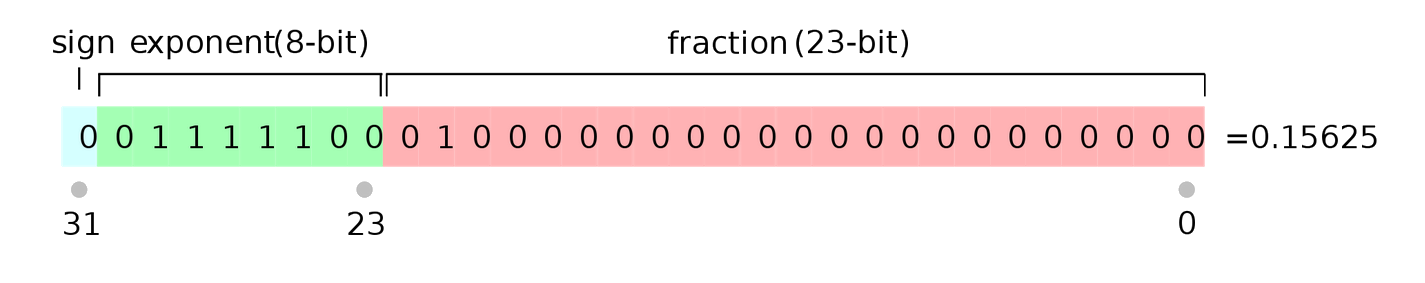
\includegraphics[scale=0.4]{images/single-precision.png} 
     	\vspace*{-0.5em}
		\caption{8 bits for exponent part, 23 bits for fraction part and 1 bit for sign}
	\end{figure}
	\end{center}	
	
	\begin{itemize}
	\item{exponent part = real exponent + 127 (in binary)
		\begin{itemize}
			\item{127 is a bias to handle negative exponents}
		\end{itemize}	
	}		
	\item{fraction part = fraction part (in binary)}
	\item{sign part = 0 (if positive) or 1 (if negative)}
	\item{\textbf{$number\ (in\ binary) = (-1)^{sign} \times 1 \times fraction\ (in\ binary) \times 2^{real\ exponent}$}} 	
	\end{itemize}		
	
	}	
	
	\end{itemize}	 
			
	\end{frame}		  

	\begin{frame}
	\begin{itemize}
		\item{Example of a real in IEEE-754 Single Precision binary representation: 
			\begin{itemize}
				\item{$23.375 = (10111.011)_2 = (-1)^0 \times 1.0111011 \times 2^{-4}$}
				\item{sign part = $0_2$}
				\item{fraction part = $(011101100000000000000000)_2$}
				\item{exponential part = $(00000100)_2 + (10000000)_2 = (10000100)_2$}
				\item{Final bit storage = $(01000010001110110000000000000000)_2$}
			\end{itemize}							
		}
	\end{itemize}			
	
	\begin{itemize}
		\item{IEEE-754 Double Precision:
		\begin{center}
		\begin{figure}
		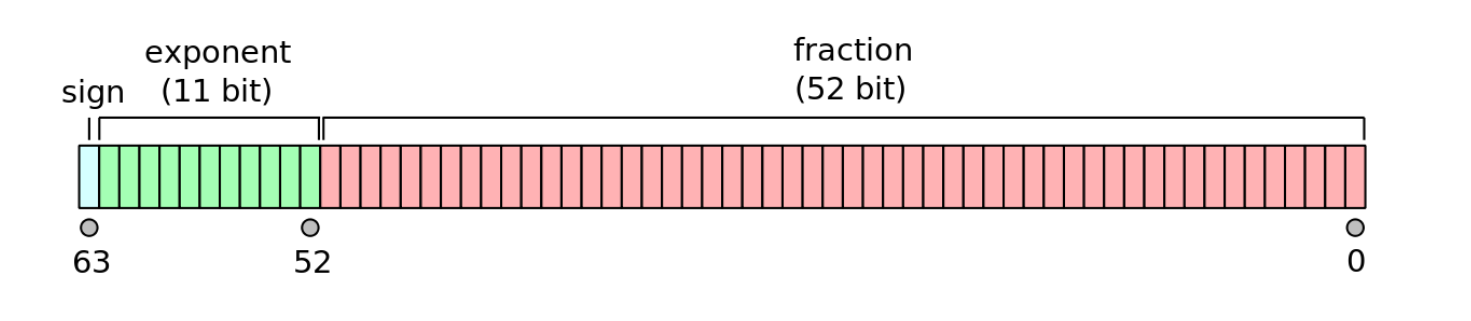
\includegraphics[scale=0.4]{images/double-precision.png} 
     	\vspace*{-0.5em}
		\caption{11 bits for exponent part, 52 bits for fraction part and 1 bit for sign}
		\end{figure}
		\end{center}	
	
		\begin{itemize}
		\item{exponent part = real exponent + 1023 (in binary)
		\begin{itemize}
			\item{1023 is a bias to handle negative exponents}
		\end{itemize}	
		}		
		\item{fraction part = fraction part (in binary)}
		\item{sign part = 0 (if positive) or 1 (if negative)}
		\item{\textbf{$number\ (in\ binary) = (-1)^{sign} \times 1 \times fraction\ (in\ binary) \times 2^{real\ exponent}$}} 	
		\end{itemize}		
	
		}	
	\end{itemize}		
		
	\end{frame}		  
		  
		  
	\subsection{Encoding characters}	
		  
	\begin{frame}
	
	Dealing with encoding characters:
	\vspace*{0.6em}	
	
	\begin{itemize}	
	\item{We know how integers and floating numbers are stored, but what about characters?}	
	\item{Indeed, characters cannot be directly transformed into bits (such as integers or floating number).}
	\item{And all information need to be transformed into bits to be processed by a computer...}	
	\item{We need an \textbf{encoding mechanism} to transform characters into bits.}
	\end{itemize}
	
	\end{frame}

	\begin{frame}
	
	What is encoding? Encoding the information consists in matching symbols to binary representations (code words) using an encoding map.
	\vspace*{0.5em}
	
	In the given example below the information is made of alphanumerical characters\footnote{it is a bijection}:	
		\vspace*{1em}
	
	\begin{center}	
	\begin{figure}
		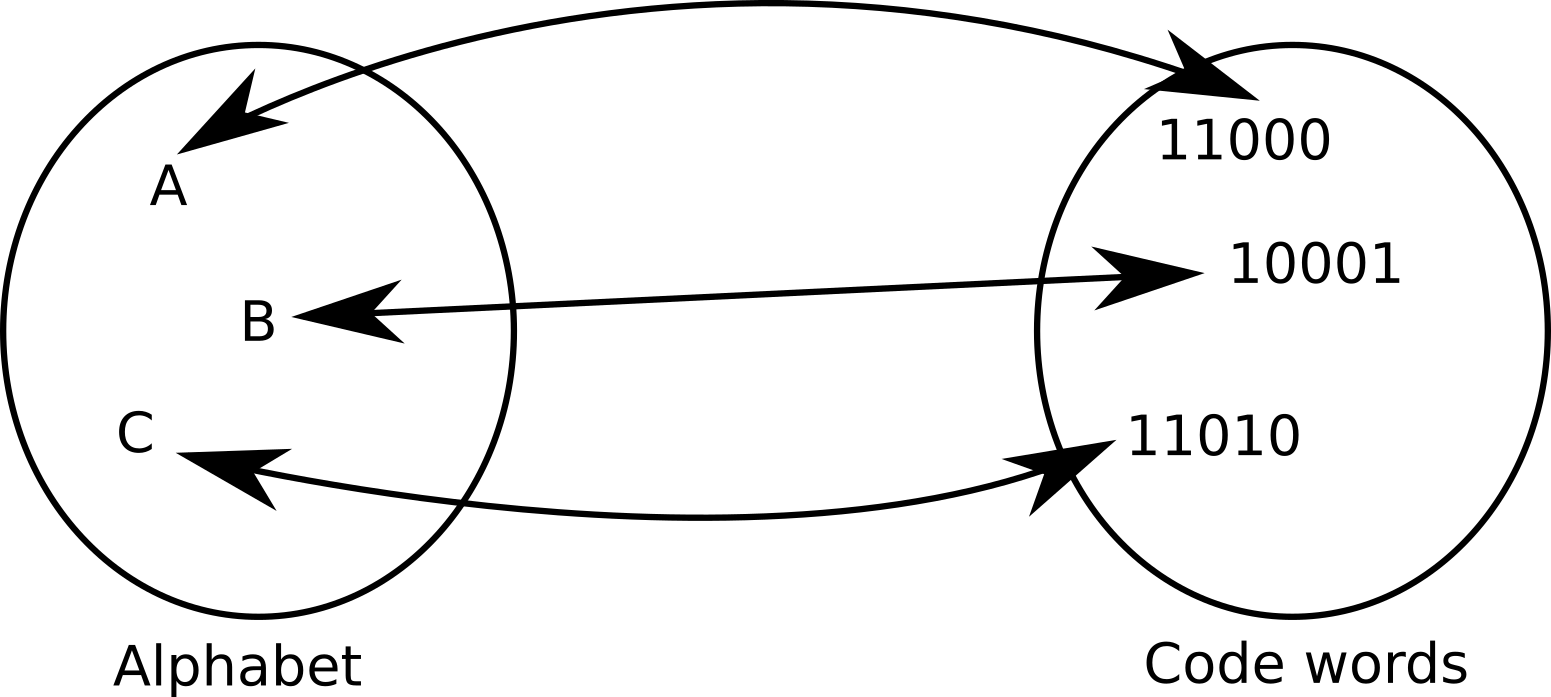
\includegraphics[scale=0.3]{images/encoding.png} 
     	%\vspace*{-0.5em}
		%\caption{Floating gate transistor cell}
	\end{figure}	
	\end{center}
		
	\end{frame}

	\begin{frame}
	
	How to get an encoding map of code words?
	\vspace*{0.6em}
	
	We can consider the character space as a system and each character as a state in this system. And we can use a fixed-state coding approach to get an encoding map:
	
	\vspace*{0.6em}	
	
	\begin{itemize}
	\item{Each state of the system is coded by a certain number of bits (called length of code) with:
		\begin{itemize}
			\item{1 bit: we can code 2 states (0 or 1)}
			\item{2 bits: we can code 4 states (00, 01, 10, 11)}
			\item{N bits: we can code $2^N$ states}
		\end{itemize}
	}	
	
	\end{itemize}
	
	The number of states required to code $P$ states is $n$ such as: 
	$2^{(n-1)} < P \leq 2^n$  	
		\vspace*{1em}	
	
	Example: We have 26 letters in the alphabets, how many bits are necessary to code $P$ values?
	We need 5 bits, because: $2^4 < 26 \leq 2^5$	
	
	
	\end{frame}
	
	
	\begin{frame}

	Examples of character encoding systems:
		\vspace*{1em}	
	
	\begin{itemize}
	
	\item{The \textbf{Baudot code} is encoded on 5 bits. With the Baudot code we can code up to 32 characters (and thus the 26 letters of the alphabet).}
	\item{The \textbf{ASCII table} (7 bits encoding). With the ASCII table uppercase letters, system and special characters can also be encoded (we can code 128 characters).}
	
	\end{itemize}
	
		
	\begin{center}	
	\begin{figure}
		\includegraphics[scale=0.2]{images/ascii_table.png} 
     	%\vspace*{-0.5em}
		%\caption{Floating gate transistor cell}
	\end{figure}	
	\end{center}		
	
	
	\end{frame}

	\begin{frame}
	
	\textbf{ASCII to unicodes:}
		\vspace*{1em}	
	
	With ASCII we can code only 128 characters...
		\vspace*{0.5em}	
	
	With ISO-8859-X (coded on 8bits) other 128 characters can be used to code for other characters (because of the 8-th bit). Other characters specific to languages such as: latin, cyrillic, arabic, greek and hebrew can be encoded as well. 
	\vspace*{0.5em}		
		
	Example of ISO-8859-X unicode: ISO-8859-1.
	\vspace*{0.5em}	
	
	With ISO-8859-X unicodes it's not possible to encode Chinese characters. The Guobiao character encoding permits that (for simplified characters: GB2312, GB13000, GB18030, GBK, GB\_1988-80 and GB\_198880, for traditional characters:  BIG-5, BIG-FIVE, BIG5-HKSCS, BIG5, BIG5HKSCS, BIGFIVE, CN-BIG5, CN-GB and CN).		
		
	
	\end{frame}
	
	\begin{frame}
	
	Examples:
	\vspace*{0.6em}
	
	\begin{itemize}
		\item{Let's imagine we have a book written in English with 150 pages and with an average of 1000 characters per page. What would be the approximate size of the specific content of this book? We can use ASCII encoding (because English)...
			\begin{itemize}
				\item{Approximate size = $150 \times 1000 \times 7$ bits = 131250B = 131.250KB}
			\end{itemize}
		 }
		\item{The same book but written in French (same average number of characters and 1.2 times more pages. And we use ISO-8859-1 encoding.)
			\begin{itemize}
				\item{Approximate size = $180 \times 1000 \times 8$ bits = 180000B = 180KB}
			\end{itemize}					
		}	
		\item{The same book written in simplified Mandarin Chinese (this time with 80 pages and an average 2000 characters per page). We use GB 18030 encoding (4 bytes per character).
			\begin{itemize}
				\item{Approximate size = $80 \times 2000 \times 4$ bytes = 640000B = 640KB}
			\end{itemize}
		}
	\end{itemize}		

	\end{frame}

	\subsection{How to deal with images, audio and video}

	\begin{frame}

	How to deal with images, audio and videos?
	
	\vspace*{0.6em}
	
	\begin{itemize}
		\item{Images, audio and videos are all continuous information.}
		\item{However, computers can only deal with discrete binary information.}
		\item{To store these information we have to \textbf{sample the continuous information into discrete values} and \textbf{transform these values into bits}.}
	\end{itemize}

	\end{frame}
	
	\begin{frame}
	
	How do we transform a continuous signal into bits?
	\vspace*{0.6em}	
	
	The continuous signal has to be transformed into a string of bits to be stored in the memory by \textbf{sampling the signal}. 
	\vspace*{0.6em}		
	
	The sampling of a continuous signal can be made by extracting samples at regular times:
	
	\begin{itemize}
	\item{The sampling interval is constant (= we have a fixed sampling frequency)}
	\item{The order of magnitude is kept}
	\item{Each sample is finally transformed into binary}
	\end{itemize}
	
	\end{frame}
	
	\begin{frame}	
	
	\begin{center}	
	\begin{figure}
		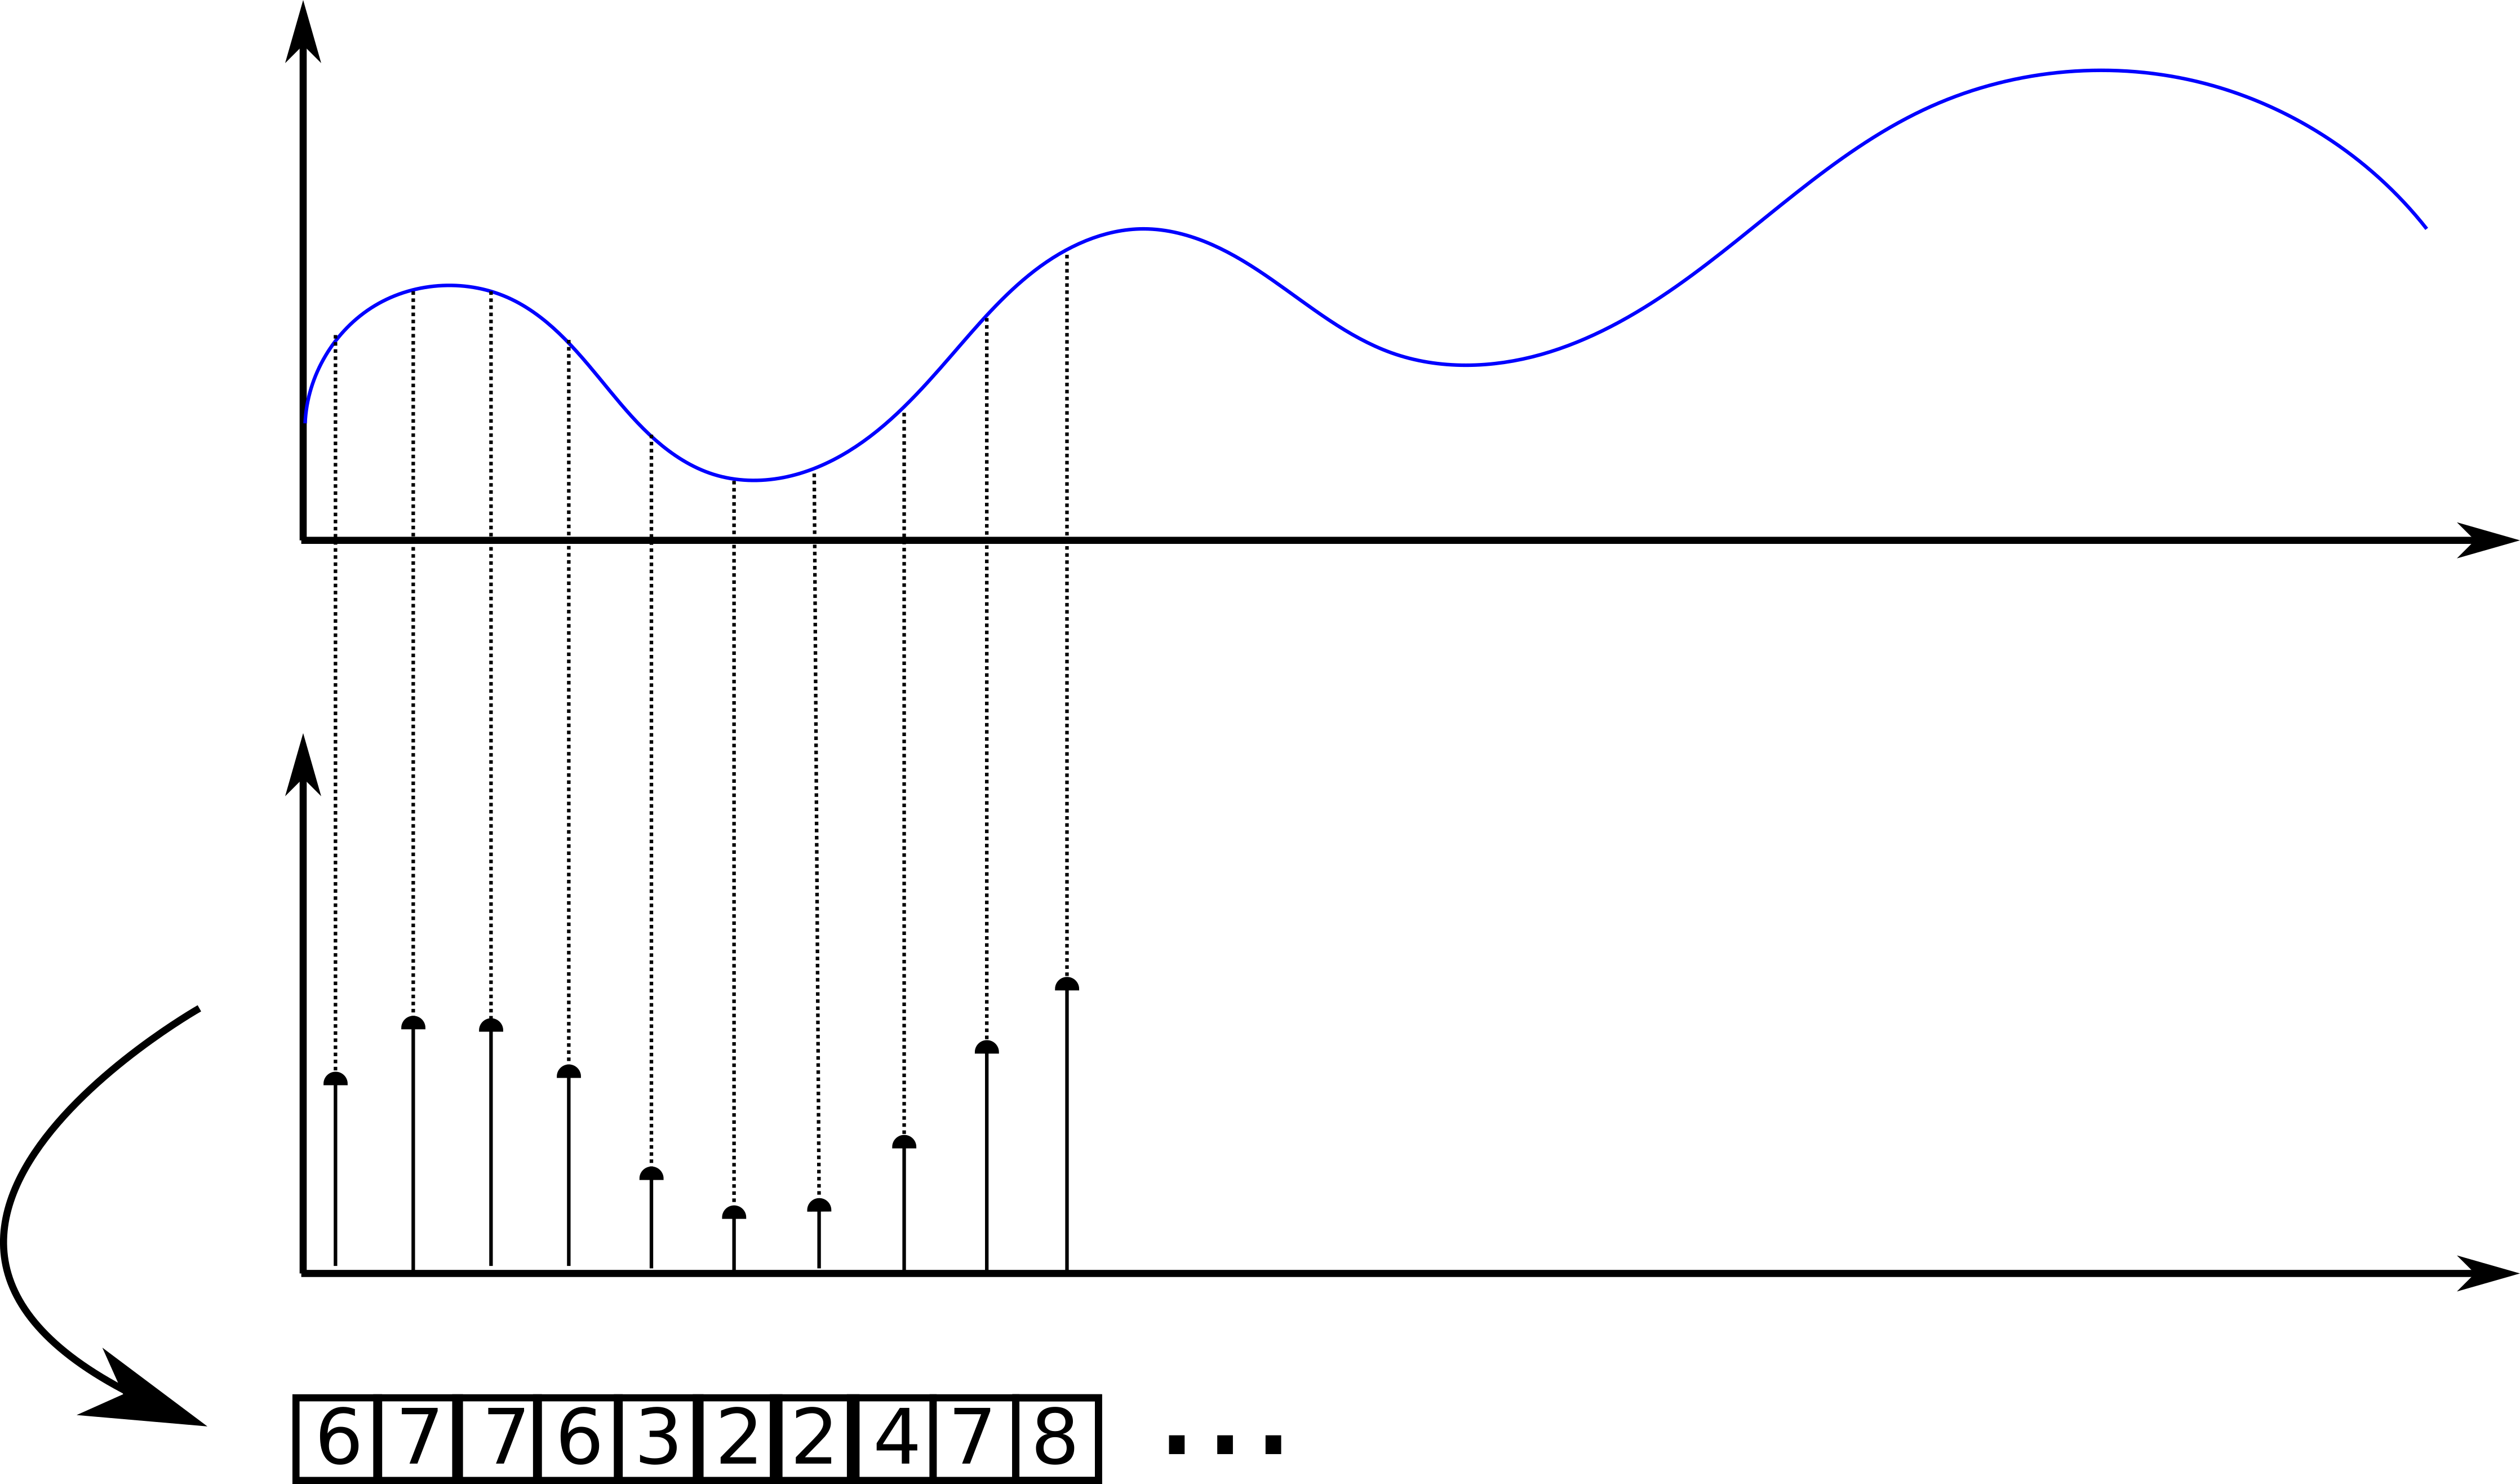
\includegraphics[scale=0.1]{images/digit.png} 
     	%\vspace*{-0.5em}
		%\caption{Floating gate transistor cell}
	\end{figure}	
	\end{center}
	\vspace*{0.5em}	
	 
	
	
	\begin{alertblock}{Beware}
	Shannon Law: the \textbf{sampling frequency must be bigger or equal to twice the maximum frequency of the signal}.	In order not to lose information.
	\end{alertblock}
		
	
	\end{frame}
	
	\begin{frame}
	
	Example 1:
	\vspace*{1em}	
	
	The max frequency of the human voice is between 300Hz and 3400Hz.
	\vspace*{0.5em}	
	
	Let's choose $F_{max}=$4000Hz
	\vspace*{0.5em}	
	
	According to the Shannon law, $F_{sampling}$ must be $\geq 2\times F_{max}$
	\vspace*{0.5em}	
	
	So let's choose $F_{sampling}=$8000Hz (8000 samples per seconds)
	\vspace*{0.5em}	
	
	Besides, to get a correct audio reproduction each sample should be encoded on 12 bits.
	\vspace*{0.5em}	
	
	So, in order to store in real time the human voice we should have a Bit Rate of $8000\times 12=$ 96000 bits/second 	
	\vspace*{0.5em}	
	
		
	\end{frame}

	\begin{frame}

	Example 2:
	\vspace*{1em}	
	
	As you know, the color can be decomposed into three different primary colors (red, green and blue).
	\vspace*{0.5em}	
	
	The weighted sum of these three primary colors give the color (this is the additive synthesis).
	\vspace*{0.5em}	
	
	 \begin{center}	
	\begin{figure}
		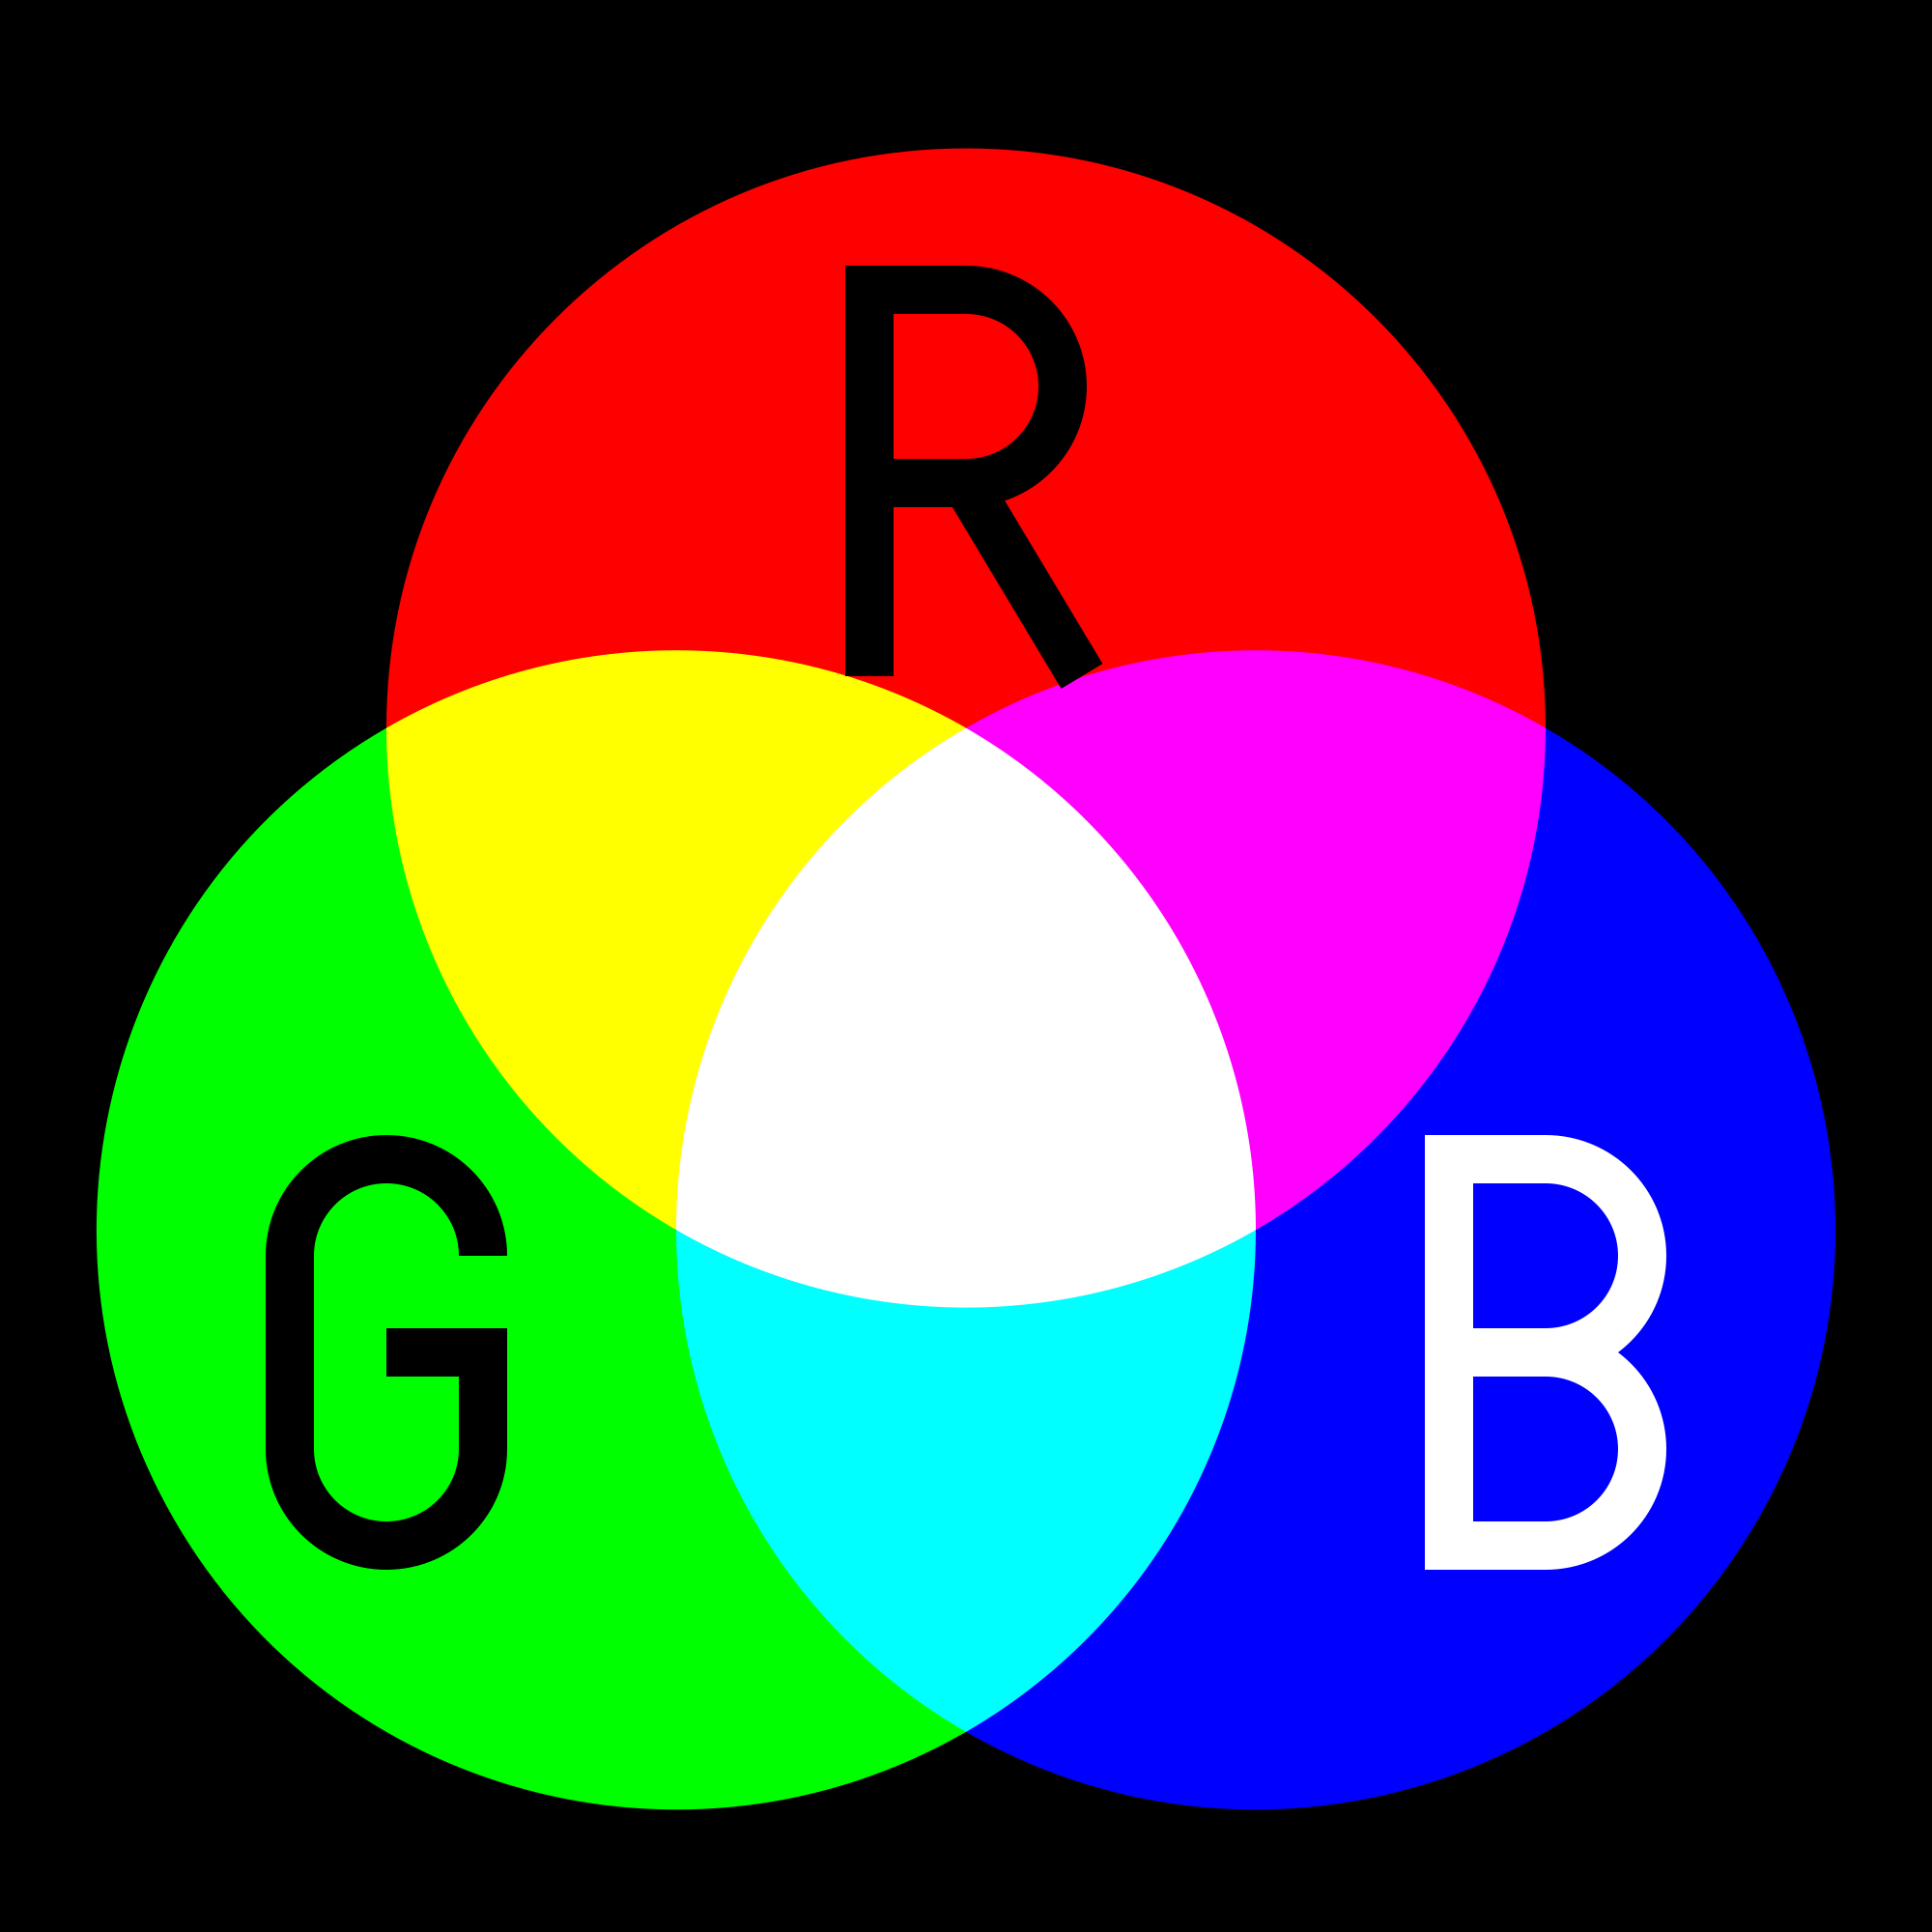
\includegraphics[scale=0.05]{images/additive.png} 
     	%\vspace*{-0.5em}
		%\caption{Floating gate transistor cell}
	\end{figure}	
	\end{center}
	
	
	\end{frame}

\begin{frame}
	
	Each image point in an image is represented  by two values: the luminance (luminious intensity) and the chrominance (conveying color information).
	\vspace*{1em}	
	
	
	These two values are bounded together by this relation:
	\vspace*{0.5em}		
	
	$Y=0.3\times R + 0.59\times V + 0.11\times B$
	\vspace*{0.5em}	
	
	Y: luminance
	R, G and B: chrominance components
	\vspace*{0.5em}	
		
		
	For example, with the lowest quality of European Digital TV standard we have:
	\vspace*{0.5em}	
	
	\begin{itemize}
	\item{625 lines per image (576 lines are really used).}
	\item{720 points per line}
	\item{25 images/second}	
	\end{itemize}			
	\vspace*{0.5em}	
		
	\end{frame}
	
	\begin{frame}
	
		
	Thus we can store:	
	\vspace*{1em}	
		
	\begin{itemize}
	\item{720 points per line for the luminance (encoded on 8bits)}
	\item{360 points each for the blue and red chrominance (encoded on 8bits)}
	\end{itemize}	
	\vspace*{0.5em}		
	
	So we have 1440 points per line.
	\vspace*{0.5em}	
	
	Number of bits to store for one image = $(1440\times 8\times 576)	= 6635520$ bits
	\vspace*{0.5em}	
	
	With a framerate of 25 images/second:
	The Bit Rate must be: $6635530\times 25=166$Mbit/s
	\vspace*{0.5em}	
		
	Actually this Bit Rate is difficult to realize, one solution is to compress the data to lower the required Bit Rate.
	\vspace*{0.6em}
	
	This is the goal of the "Motion Picture Expert Group" or MPEG: they define the compression algorithm for sound and video (see after in the course for more info about compression)...		
		
	\end{frame}
	
	\section{File formats}	
	
	\begin{frame}
	
	On computers, data is mostly stored on files. 
	\vspace*{0.6em}
	
	We have two categories of file formats: \textbf{binary} and \textbf{text} file formats:
 	 	
	\begin{itemize}
		\item{Binary file formats: 
				\begin{itemize}
					\item{Can store multiple types of information in a single file (audio, text, video). Example: xlsx}
					\item{Very application dependent (mostly, only Excel can read xlsx, you cannot open avi file with Excel, etc)}
					\item{Here 1 byte = 1 custom data (huge byte sequence dependency)}
				\end{itemize}				
		 }
		\item{Text file formats: 
			\begin{itemize}
				\item{Encoding dependent (ASCII, ISO-8859-1, GB18030, etc)}
				\item{Can be opened on any system by any editor}
				\item{Easy to read and understand}
				\item{Less prone to get corrupted, more robust (1 byte error = may be just one error on an isolated and non important character)}
				\item{1 byte = 1 readable character}
			\end{itemize}							
		}
	\end{itemize}
		
	\end{frame}		
		
	\begin{frame}
	
	A non-exhaustive list of interesting file formats in Data Engineering:
	\vspace*{0.6em}	

	\begin{itemize}
		\item{CSV, TSB: column and tab-based text file formats}
		\item{XLSX XLS: sheets+columns+media binary Excel file format}
		\item{JSON: key-value-based structured file format}
		\item{XML: tag-based structured file format}
		\item{AVRO: Hadoop binary dump file format}
		\item{PARQUET: column first binary file format}
		\item{JPG, PNG and so on: image binary file formats}
		\item{MPEG, OVG and so on: video binary file formats}
		\item{MP3 and so on: audio binary file formats}
		\item{Many other...}
	\end{itemize}
	
	\end{frame}	

	\begin{frame}[fragile]
	
	CSV (Comma Separated Value) - Text file
	\vspace*{0.6em}
	
	\begin{itemize}
		\item{A CSV is a file with the values comma-separated, this is used to store column and row data}
		\item{CSV files can be used with Microsoft Excel, Google Spreadsheets, etc}
		\item{It differs fron other spreadsheet format: you can only have one single sheet in a file. You cannot store formulas, images, etc.}
	\end{itemize}		
	
	CSV file exemple:
	\begin{verbatim}
	column_name_1, colum_name_2, column_name_3, ...
	value1, value2, value3, ...
	\end{verbatim}

	Code exemple (python/pandas):
	\begin{verbatim}
	import pandas as pd
	data = pd.read_csv(sep=",", "example.csv")
	print(data['column1'])
	\end{verbatim}

	Code exemple (awk):
	\begin{verbatim}
	awk -F',' '{ print $1; }'
	\end{verbatim}

	\end{frame}
	\begin{frame}[fragile]
	
	TSV (Tabular Separated Value) - Text file
	\vspace*{0.6em}	

	\begin{itemize}
		\item{Values are tab-separated}
		\item{TSV is an alternative to the common comma-separated values (CSV) format}
		\item{CSV: difficulties if you use commas in values...}	
	\end{itemize}		

	Exemple:
	\begin{verbatim}
	column_name_1	column_name_2	column_name_3	...
	value1	value2	value3	...		
	\end{verbatim}

	Code (using Python/pandas):
	\begin{verbatim}
	import pandas as pd
	data = pd.read_csv(sep="t", "example.csv")
	print(data['column1'])
	\end{verbatim}
 	
 	Code (using awk):
 	\begin{verbatim}
 	awk -F'\t' '{ print $1; }'	
 	\end{verbatim}
 	
	\end{frame}
	\begin{frame}[fragile]
	XLSX, XLS (Excel file format) - Binary format
	\vspace*{0.6em}
	
	\begin{itemize}
	\item{Official spreadsheet format of Microsoft Excel}
	\item{Store column/raw data in sheets}
	\item{Can store more than one sheet, plus images, videos, etc.}
	\end{itemize}
	\vspace*{0.6em}

	Code (using pandas):
	\begin{verbatim}
	import pandas
	data = pd.ExcelFile('example.xls')
	df1 = pd.read\_excel(data, 'my sheet 1')
	df2 = pd.read\_excel(data, 'my sheet 2')	
	\end{verbatim}
			
	\end{frame}
	\begin{frame}[fragile]
	
	JSON (JavaScript Object Notation) - Text format
	\vspace*{0.6em}
	
	\begin{itemize}
	\item{Data are stored and structured as attribute-value pairs}
	\item{Returned format of some APIs (Application Programming Interface)}
	\item{Open standard file format}
	\end{itemize}		
	
	Exemple:
	\vspace*{0.6em}
	
	\begin{verbatim}
	{ "sport": {
            "ball": {
                "solo": ["tennis",	"pingpong"],
                "team": ["soccer", "rugby"]
              }
    }}
	\end{verbatim}
	Code (using pandas):
	\begin{verbatim}
		import json
		data = json.load(open("example.json")
		print(data['sport']['ball'])	
		print(data['sport']['ball']['solo'])	
	\end{verbatim}
	
	\end{frame}
	\begin{frame}[fragile]
	
	XML (eXtensive Markup Language) - Text format	
	
	\vspace*{0.6em}
	\begin{itemize}
	\item{Format used to structure data for storage and transport}
	\item{The structure is made of tags, options and clear text}
	\item{This is the returned type of some APIs (ex: WeChat API)}	
	\end{itemize}
	
	Exemple:
	\begin{verbatim}
	<?xml version="1.0" encoding="UTF-8"?>
	<email>
	  <from>Jani</from>
	  <body>Message 1</body>
	</email> 
	\end{verbatim}		
	
	Code example (Python):
	\begin{verbatim}
	import xml.etree.ElementTree as ET 
	tree = ET.parse("example.xml")
	root = tree.getroot() 
	item = root.find("email")
	\end{verbatim}
	
	\end{frame}
	
	\begin{frame}[fragile]
	Parquet - Binary format
	\vspace*{0.6em}
	
	\begin{itemize}
		\item{Designed for large-scale analytical querying}
		\item{A flat columnar storage format (different than CSV/TSB that are row-based)}
		\item{Designed to bring efficiency
			\begin{itemize}
				\item{Row-based easier to conceptualize, but slower to use in some case}
				\item{Column-based permits to skip non-relevant data quickly} 
			\end{itemize}					
		}
	\end{itemize}
			
	\begin{center}	
	\begin{figure}
		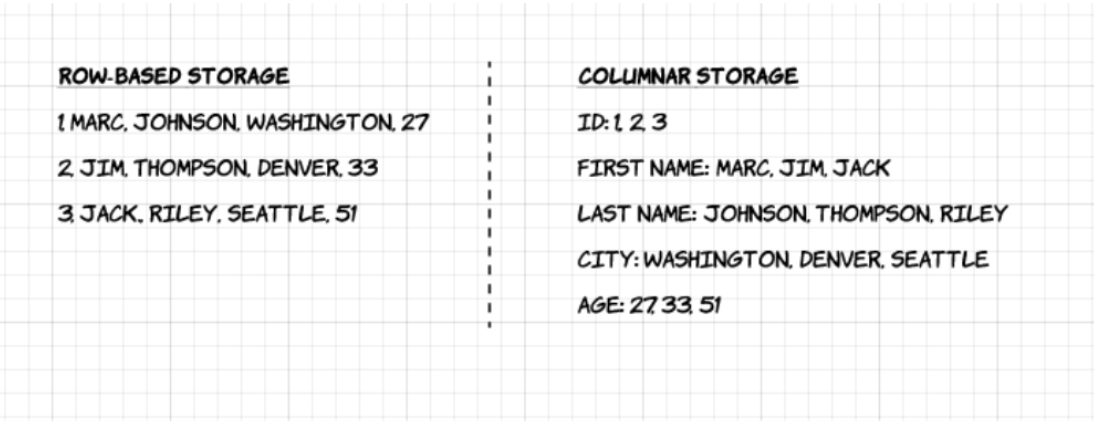
\includegraphics[scale=0.4]{images/parquet.png} 
     	%\vspace*{-0.5em}
		%\caption{Floating gate transistor cell}
	\end{figure}	
	\end{center}
	
	Code example (Python):
	\begin{verbatim}
	import pyarrow.parquet as pq
	pq.write_table(table, 'example.parquet')	
	\end{verbatim}
	
	\end{frame}
	\begin{frame}[fragile]	
	Pickle (Serialized format) - Binary format
		
	\vspace*{0.6em}
	\begin{itemize}
		\item{Serialization refers to the process of converting object from the main memory to the disk}
		\item{Pickle is a well-known Python module permitting that}
		\item{Very useful to store objects, structures or Machine Learning models}
	\end{itemize}		
	
	Code exemple:
	\begin{verbatim}
	import pickle
	class exampleClass:
    	a = 35
    	b = [1, 2, 3]
	object = exampleClass()
	outfile = open("example.bin",'wb')
	pickled_object = pickle.dump(object, outfile) 
	infile = open("example.bin", 'rb')
	loaded_pickled_object = pickle.load(infile)
	\end{verbatim}
		
	\end{frame}
	\section{Databases}
	
	\begin{frame}
	
	Another popular way to save data is to store it in a \textbf{database}.	
	\vspace*{0.6em}	
	
	What is a database?
	\vspace*{0.6em}
	
	\begin{itemize}
	\item{Alternative at storing data in the file system}
	\item{An elegant way to \textbf{centralize all the data in one place}}
	\item{Force users and developers to access and store the data in \textbf{a unique and well defined way}}
	\item{Permit to \textbf{structure the data and manage it in a powerful way}}
	\item{\textbf{Different levels of permission} can be set
		\begin{itemize}
			\item{Administrator can read, write and delete everything}
			\item{Users can only access their databases and in a specific way}
		\end{itemize}			
	}

	\item{Databases usually \textbf{offer a set of very powerful functionality to extract and write data}
		\begin{itemize}
			\item{Accessible through a language (SQL), an API and/or the command line}
			\item{Can be directly "plugged" to a software}
		\end{itemize}
	}
	\end{itemize}
	
	\end{frame}	
	
	\begin{frame}

	Example of a relationship diagram of a relational database:
	\vspace*{0.6em}
	
	\begin{center}	
	\begin{figure}
		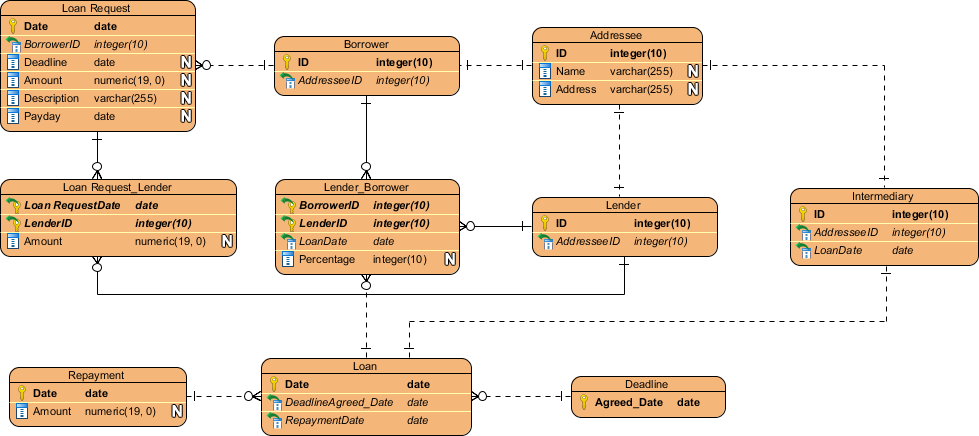
\includegraphics[scale=0.3]{images/relational-database.png} 
     	%\vspace*{-0.5em}
		%\caption{Floating gate transistor cell}
	\end{figure}	
	\end{center}
 		
	\end{frame}
		
		
	\begin{frame}	
	Actually, there are two main types of databases:
	
	\vspace*{0.6em}
	\begin{enumerate}
		\item{Relational Databases (using the SQL language)
			\begin{itemize}
				\item{MySQL: Relatively easy to use, suitable for most applications}
				\item{PostgreSQL: Complex to use, but more powerful than MySQL}
				\item{SqLite: Easy to use}
				\item{Etc.}		
			\end{itemize}			
		}
		\item{Non-relational Databases called NoSQL
			\begin{itemize}
				\item{MongoDB}
				\item{ElasticSearch}
				\item{Etc.}	
			\end{itemize}
		}	
	\end{enumerate}
	\end{frame}
	
	\begin{frame}
	
	Comparisons between Relational and Non-Relational databases:
	\vspace*{0.6em}
	
	\begin{center}
	\resizebox{\columnwidth}{!}{
	\begin{tabular}{c | c | c }
	Property &	Relational Databases  &	 Non-Relational Databases \\ \hline
	Data model & Relational & Non-relational \\ \hline
	Structure &	Table-based, with columns and rows & Document based, key-value pairs, graph, or wide-column \\ \hline
	Schema & A predefined and strict schema in which every record (row) & A dynamic schema, records don't need to be of same nature \\ \hline
	Query language & Structured Query Language (SQL) & Varies from database to database \\ \hline
	Scalability & Vertical & Horizontal \\ \hline
	Ability to add new properties & Need to alter the schema first (migration: risky!) & Possible without disturbing anything \\ \hline	
	\end{tabular}
	}
	\end{center}	
	
	\end{frame}	
	
	\begin{frame}[fragile]
	Code example (Python and SQLite - a relational database):
	\vspace*{0.6em}
	
	\begin{verbatim}
	import sqlite3
	conn = sqlite3.connect('mydatabase.db')
	cursor = conn.execute("SELECT id, name, address, salary from COMPANY")
	for row in cursor:
   		print("NAME = {}".format(row[1]))
   		print("SALARY = {}".format(row[2]))   		
 	conn.close() 		
	\end{verbatim}
 	
	Code example (Python and MongoDB - a non-relational database):
	\vspace*{0.6em}

	\begin{verbatim}
	from pymongo import MongoClient
	client = MongoClient(host="localhost", port=27017)
	db = client["mydb"]
	collection = db.addresses
	address = collection.find_one({"NAME": "Jon"})
	collection.insert_one({"NAME": "Paul", "PHONE": "12334"})	#JSON format here!
	client.close()
	\end{verbatim}

	\end{frame}
	
	\section{Data compression}
	
	\begin{frame}
	
	Data Compression, what is it and why we need it in Data Engineering?
	\vspace*{0.6em}	
	
	\begin{itemize}
		\item{Data Compression: process of encoding information using fewer bits than the original representation}
		\item{We need it to:
			\begin{itemize}
				\item{Save transmission capacity}
				\item{Save transmission time}
				\item{Reduce storage occupancy}
				\item{Reduce computation}	
			\end{itemize}					
		 }
		\item{So it's all about saving resources and money...}
	\end{itemize}
	\vspace*{0.6em}
	
	Basically two main types of compression:
	\vspace*{0.6em}
	
	\begin{itemize}
		\item{Lossy compression}
		\item{Lossless compression}
	\end{itemize}		
	
	\end{frame}
	
	\begin{frame}
	
	Examples of popular algorithms used for compressing data:
	\vspace*{0.6em}	
	
	Lossless algorithms:
	\begin{itemize}
		\item{Run-length}
		\item{Huffman (used with: zip, gzip, png, etc.)}
		\item{LZW (Lempel-Ziv-Welch) (used with: gif, tiff)}
		\item{LZMA (Lempel-Ziv-Markov chain algorithm) (used with 7zip)}
		\item{Etc.}		
	\end{itemize}
	
	Lossy algorithms:
	\begin{itemize}
		\item{JPEG (images)}
		\item{MPEG (videos)}
		\item{MP3 (audio)}
	\end{itemize}
	
	\end{frame}
	\begin{frame}
	
	What is a lossless compression?
	\vspace*{0.6em}
	
	\begin{itemize}
		\item{It means there is \textbf{no loss of information when the data is compressed}}
		\item{\textbf{Original data can be exactly recovered from the compressed data} (exact size before and after)}
		\item{Usually used with \textbf{applications that cannot tolerate a loss of information}, for example:
			\begin{itemize}
				\item{word documents}
				\item{computer programs}
				\item{company's customer dataset}
				\item{Etc.}
			\end{itemize}					
		}
		\item{Principle: 
			\begin{itemize}
				\item{\textbf{Redundant data is removed during compression}}
				\item{\textbf{Redundant data is added back during decompression...}}
			\end{itemize}			
		}		
	\end{itemize}
	
	\end{frame}	
	
	\begin{frame}

	What is a lossy compression?
	\vspace*{0.6em}
	
	\begin{itemize}
		\item{Lossy compression results in \textbf{lost data and quality from the original representation}}
		\item{However, because 	it removes data from original representation it \textbf{usually mean a greater compression}}
		\item{Remove just what have to be removed:
			\begin{itemize}
				\item{JPEG may reduce image's size by more than 80\% without noticeable effect}
				\item{MP3 may reduce down to one tenth the size of the original audio file}	
			\end{itemize}					
		}
		\item{Trade-off: \textbf{a greater compression will take up less space, but may alter the quality}}	
	\end{itemize}
	\end{frame}

	\begin{frame}
	
	In Data Engineering we are mostly interested in used lossless compression.
	Let's compare\footnotemark these lossless compression file formats then:
	\vspace*{0.6em}

	\begin{itemize}
	\item{\textbf{gzip}: uses Lempel-Ziv coding (LZ77) (tar czf pack.tar.gz rep/}
	\item{\textbf{bzip2}: uses the Burrows-Wheeler block sorting text compression algorithm and Huffman coding (tar cjf pack.tar.bz2 rep/)}
	\item{\textbf{zip}: ZIP MSDOS (zip -r pack.zip rep/)}
	\item{\textbf{rar}: proprietary archive file format (rar a pack.rar rep/)}
	\item{\textbf{lha}: based on Lempel-Ziv-Storer-Szymanski-Algorithm (LZSS) and Huffman coding (lha a pack.lha rep/)}
	\item{\textbf{lzma}: Lempel-Ziv-Markov chain algorithm (tar --lzma -cf pack.tar.lzma rep/)}
	\item{\textbf{lzop}: Similar to gzip but favors speed over compression ratio (tar --lzop -cf pack.tar.lzop rep/)}
	\end{itemize}

	\footnotetext{Original study: https://binfalse.de/2011/04/04/comparison-of-compression/}
	
	\end{frame}
	
	\begin{frame}
	
	Comparing the compression of binaries (total: 176.753.125 Bytes):
	\vspace*{0.6em}
	
	\begin{center}
	\resizebox{\columnwidth}{!}{
	\begin{tabular}{c | c | c | c }
	Method & Compressed Size & \% of original & Time in s \\ \hline
	gzip &	161.999.804 &	91.65 &	10.18 \\ \hline
	bzip2 &	161.634.685	& 91.45 &	71.76 \\ \hline
	zip &	179.273.428 &	101.43 &13.51 \\ \hline
	rar &	175.085.411 &	99.06 &	156.46 \\ \hline
	lha &	180.357.628	& 102.04 &	35.82 \\ \hline
	lzma &	157.031.052 &	\textbf{88.84} &	129.22 \\ \hline
	lzop &	165.533.609 &	93.65 &	\textbf{4.16} \\ \hline
	\end{tabular}
	}
	\end{center}	
		
	\end{frame}	
	
	\begin{frame}
	
Comparing plain text compression (total: 40.040.854 Bytes):	
\vspace*{0.6em}
	
	\begin{center}
	\resizebox{\columnwidth}{!}{
	\begin{tabular}{c | c | c | c }
	Method &	Compressed Size	 & \% of original & Time in s \\ \hline
	gzip &	11.363.931 &	28.38 &	1.88 \\ \hline
	bzip2 &	9.615.929 &	24.02 &	13.63 \\ \hline
	zip &	12.986.153 &	32.43 &	1.6 \\ \hline
	rar	& 11.942.201 &	29.83 &	8.68 \\ \hline
	lha	& 13.067.746 &	32.64 &	8.86 \\ \hline
	lzma &	8.562.968 &	\textbf{21.39} &	30.21 \\ \hline
	lzop &	15.384.624 &	38.42 &	\textbf{0.38} \\ \hline
	\end{tabular}
	}
	\end{center}	
	
	\end{frame}	
	
		
	\begin{frame}
	
	Comparing the compression of a mix of data (plain+media+binary+pictures+random, total: 355.971.825 Bytes):
	\vspace*{0.6em}	
	
	\begin{center}
	\resizebox{\columnwidth}{!}{
	\begin{tabular}{c | c | c | c }
		Method &	Compressed Size	 & \% of original & 	Time in s \\ \hline
		gzip &	294.793.255 &	82.81 &	20.43 \\ \hline
		bzip2 &	290.093.007	& 81.49 &	141.89 \\ \hline
		zip &	313.670.439	& 88.12	& 23.78 \\ \hline
		rar &	305.083.648	 & 85.70 &	246.63 \\ \hline
		lha &	315.669.631 &	88.68 &	64.81 \\ \hline
		lzma &	283.475.568	& \textbf{79.63} &	258.05 \\ \hline
		lzop &	307.644.076 &	86.42 & \textbf{7.89} \\ \hline
	\end{tabular}
	}
	\end{center}	

	\end{frame}
	
	\begin{frame}
	
	For the next courses:
	
	\begin{itemize}
		\item{Enough of the theory for now!}
		\item{Bring your laptop computer!}
		\item{You will need Linux on virtual machine: https://itsfoss.com/install-linux-in-virtualbox/}
		\item{Or installed on a USB stick: https://itsfoss.com/create-live-usb-of-ubuntu-in-windows/}		
	\end{itemize}
	\end{frame}	
	
\end{document}
